\documentclass[12pt]{report}

% Čeština
\usepackage[utf8]{inputenc}
\usepackage[IL2]{fontenc}
\usepackage[czech]{babel}

% Formát dokumentu
\usepackage{caption}
\usepackage{indentfirst}
\usepackage{graphicx}
\usepackage{textcomp}
\usepackage{amsmath}
\usepackage{parskip}
\usepackage{xspace}
\usepackage[linesnumbered,ruled,vlined]{algorithm2e}
\graphicspath{{img/}}
\usepackage[
left=30mm, 
right=30mm, 
top=30mm, 
bottom=30mm,
]{geometry}
						
\begin{document}
	{\centering
		
		\vspace{15mm}
		
		{\Huge\bfseries KIV/PRO}
		
		{\Huge\bfseries Boundary iterative deepening depth-first search}
		
		{\LARGE Mikuláš Mach - \today}
		\vspace{15mm}
		
	}
	
	\section*{Zadání}
	
	Najděte v anglicky psané odborné literatuře článek v délce alespoň 5 stránek o nějakém 
	algoritmu řešícím libovolný problém. Algoritmus popište do českého referátu tak, aby ho 
	podle vašeho názoru pochopil běžný student 2. ročníku informatiky. Váš text musí svědčit o 
	tom, že algoritmu rozumíte, a musí ho z něj pochopit i nezasvěcený čtenář. 
	
	%-----------------------
	%ÚVOD
	%-----------------------
	
	\section*{Úvod}
	
	Hledání cesty je proces nalezení cesty mezi dvěma body, které se nacházejí na mapě nebo v nějakém prostředí.
	Pro tento proces se využívají tzv. pathfinding algoritmy. Hledaná je nejčastěji ta cesta, která má nejmenší vzdálenost, nejmenší cenu nebo nejkratší čas cesty. Pathfinding algoritmy se dělí na informované a neinformované. Informované algoritmy využívají heuristickou funkci, která směruje postup prohledávání k cílovému bodu. Na rozdíl od toho neinformované algoritmy nevědí kde se cíl nachází a typicky hledají cestu ve všech směrech.
	
	V tomto referátu bude popsán neinformovaný pathfinding algoritmus \textbf{Boundary iterative deepening depth-first search} (Lim, 2015) dále BIDDFS, který kombinuje \textbf{Dijkstrův algoritmus} (Dijkstra, 1959) a \textbf{Iterative deepening depth-first search} (Korf, 1985) dále IDDFS. Díky spojení vlastností těchto algoritmů, lze BIDDFS využít na hledání nejkratší cesty v ohodnoceném grafu či mapě.
	
	\newpage
	
	\section*{Boundary iterative-deepening depth-first search}
	
	BIDDFS je algoritmus, který se zbavuje paměťové náročnosti Dijkstrova algoritmu a redundantnosti prohledávání IDDFS. BIDDFS stejně jako IDDFS používá hraniční hodnotu, která udává do jaké vzdálenosti od počátečního uzlu v jedné iteraci prohledáme daný graf/mapu, ale na rozdíl od IDDFS se po zvýšení hraniční hodnoty neprohledává graf znova od začátku, ale začíná se od hraničních uzlů, které jsou uloženy v listu. Pro nalezení nejkratší cesty se ještě musí ukládat cena cesty z počátku do daného uzlu a rodič daného uzlu, díky tomu budeme moct pomocí zpětného krokování nalézt cestu z počátku do cíle. Tento algoritmus najde stejnou cestu jako Dijkstrův algoritmus.
	
	BIDDFS postupuje tímto způsobem:
	
	\begin{description}
		\item[1)] Z listu hraničních uzlů vezme uzel a zkontroluje zda není cílový.  Pokud ano tak algoritmus končí. Pokud list hraničních uzlů je prázdný tak algoritmus taky končí. Po každém výběru se posouvá iterátor. Smyčka bodů 1-4 se opakuje tak dlouho dokud se nepřejde přes celý list, pak se přesouvá na bod 5).
		\item[2)] Jestli vzdálenost z počátku do uzlu z bodu 1) je větší než hraniční hodnota, tak se vracíme do bodu 1)
		\item[3)] Aktualizuje se vzdálenost z počátku do potomků uzlu z kroku 1).
		\item[4)] Uzel z bodu 1) odebere z listu a nahradí ho potomky tohoto uzlu. Algoritmus se vrací do bodu 1).
		\item[5)] Zvýší se hraniční hodnota a vrací se do bodu 1) kde se začne list procházet od začátku
	\end{description}
	
	
	
	Na obrázku \ref{fig:biddfs} na straně \pageref{fig:biddfs} jsou porovnány dvě po sobě jdoucí iterace algoritmu IDDFS a algoritmu BIDDFS.
	
	\newpage
	
	\begin{figure}[h]
	\centering
	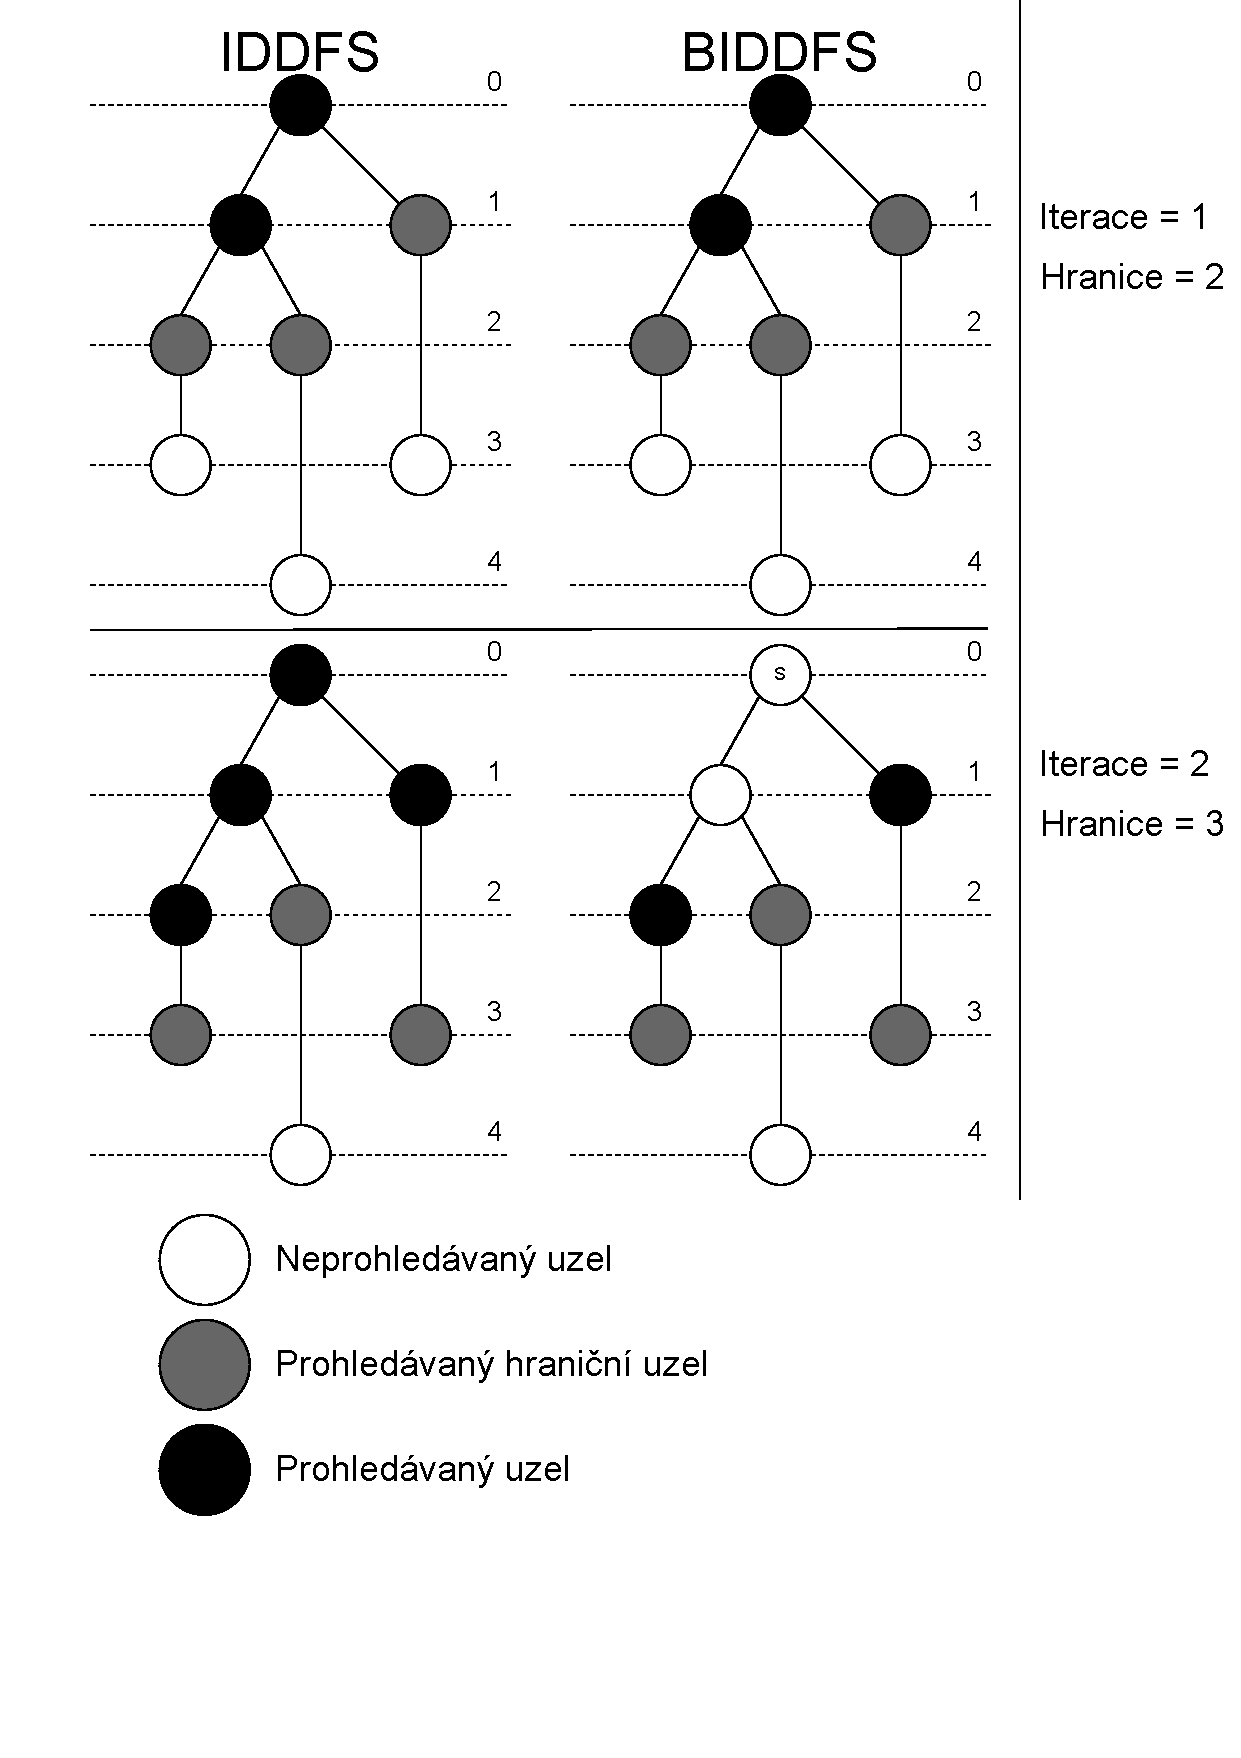
\includegraphics[width=.7\textwidth]{img/biddfs}
	\caption{Porovnání IDDFS s BIDDFS}
	\label{fig:biddfs}
    \end{figure}
	
	
	\newpage
	
	
	\section*{BIDDFS pseudokód}
	
	\begin{algorithm}
		\small
		
		\textbf{List} hraniční\_uzly = počáteční uzel
		
		\textbf{Tree} uzly[počáteční] = (vzdálenost od počátku: 0, Rodič: NULL)
		
		\textbf{bool} nalezen\_cíl = false
		
		\textbf{int} hraniční\_hodnota = 0
		
		\While{nalezen\_cíl = false \textbf{AND} hraniční\_uzly is NOT Empty }{
			
			\textbf{int} hraniční\_rozdíl = INFINITE
			
			\For{n \textbf{in} hraniční\_uzly \textbf{from} left \textbf{to} right}{
			
				(g, rodič) = uzly[n]
			
				\If{g\textgreater hranicni\_hodnota}{
				
					hraniční\_rozdíl = min(g, hraniční\_rozdíl)	
				
					\textbf{continue}
		}
	
				\If{n = cíl}{
					nalezen\_cíl = true
					
					\textbf{break}	
			}
			//funkce childrens vrátí potomky daného uzlu
			
			\For{c \textbf{in} childrens(n) \textbf{from} right \textbf{to} \textbf{left}}{
		
				//dinstance\_between vrátí cenu hrany mezi uzlem n a jeho potomkem c
				g(c) = g + distance\_between(n, c)
				
				\If{uzly[c] != NULL}{
			((g´, rodič)) = uzly[c]
	
				\If{g(c)\textgreater=g´}{
					\textbf{continue}
			}
				//vloží potomka c do listu za uzel n
				
				\textbf{insert} c \textbf{in} hraniční\_uzly \textbf{past} n
				
				//přiřadí potomkovy cenu cesty od startu a rodiče n
				
				uzly[c] = (g(c), n)				
			}
	}
		\textbf{remove} n from hraniční\_uzly
		}
			hraniční\_hodnota = hraniční\_rozdíl
		}
	\If{nalezen\_cíl = true}{
	//najde nejkratší cestu 
	
	\textbf{make} path \textbf{from} uzly
}
		\caption{BIDDFS}
	\end{algorithm}
	
	\newpage
	
	\section*{BIDDFS a obousměrné prohledávání}
	
	Obousměrné prohledávání je založeno na tom, že známe pozici cíle a to nám umožňuje prohledávat zároveň z cíle i z počátku. V tomto případě vždy provedeme jednu iteraci BIDDFS s určitou hraniční hodnotou ze startovací pozice a poté s určitou hodnotou z cílové pozice. Cyklus se bude opakovat dokud se cesty nestřetnout, poté pro nalezení cesty se bude muset provést zpětné krokování dvakrát a to vždy od místa střetu k cílové pozici a pak od střetu k počáteční pozici. Pro kontrolu střetu cesty od počátku a cesty od konce bude zapotřebí přidat 2D pole, které bude mít stejné rozměry jako prohledávaná mapa. Na každém indexu bude zaznamenáno odkud do daného políčka bylo přistoupeno, například 1 bude reprezentovat přistup od počátku, 2 bude reprezentovat přístup od z cílové pozice a 0 bude ještě neprohledané políčko. Střetnutí cest zastaví algoritmus a vrátí nejkratší cestu.
	
	Obousměrné prohledávání je teoreticky rychlejší a šetrnější na paměť než jednosměrné prohledávání. Na obrázku \ref{fig:bbiddfs} na straně \pageref{fig:bbiddfs} je porovnání jednosměrného a obousměrného BIDDFS. Z obrázku je vidět že obousměrné prohledávání prohledalo méně uzlů.
	
	
	\begin{figure}[h]
		\centering
		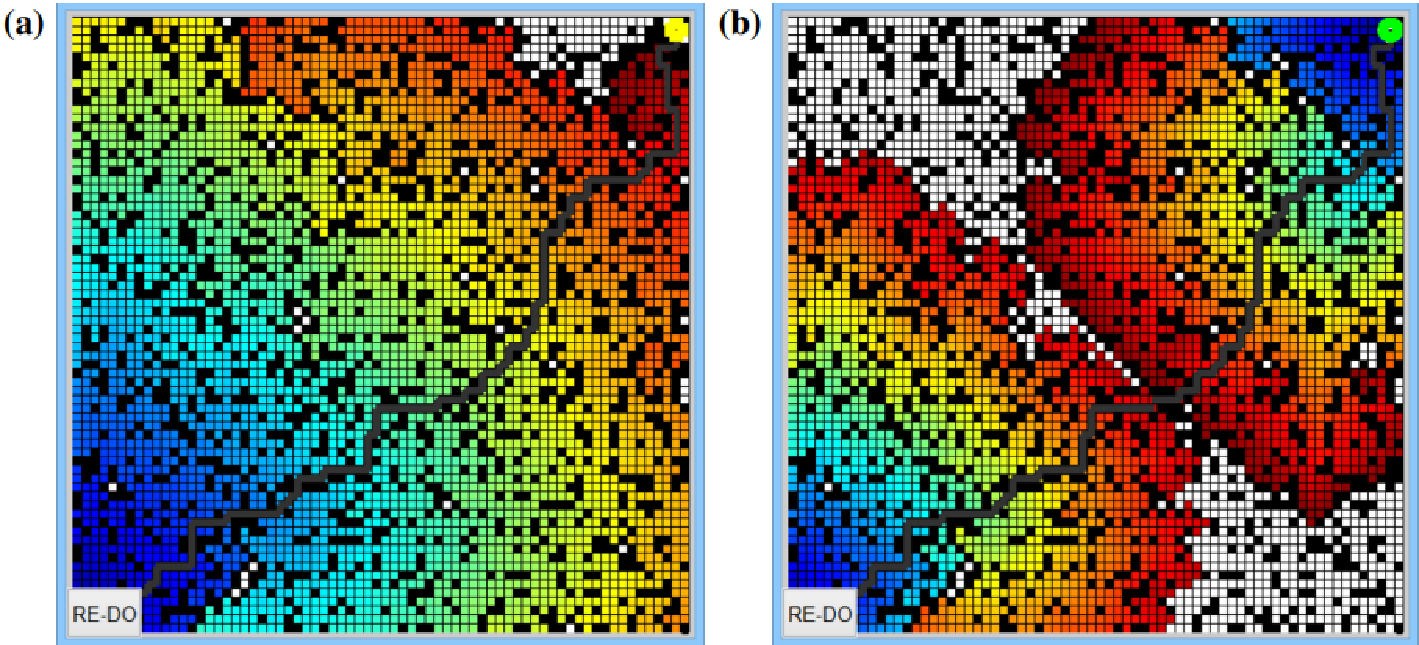
\includegraphics[width=1\textwidth]{img/bbiddfs}
		\caption{porovnání a)BIDDFS a b)obousměrného BIDDFS (Lim, 2015)}
		\label{fig:bbiddfs}
	\end{figure}
	
	Obousměrné prohledání se v tomto případě dá vylepšit pomocí paralelního prohledávání. Obousměrné BIDDFS bude rozděleno do tří vláken. Hlavní vlákno bude obsahovat 2D pole pro kontrolu zda se cesty nepotkaly a zároveň nastartuje další dvě vlákna. Ve zbytku vláken bude z každého směru spuštěno prohledávání. Když hlavní vlákno detekuje setkání cest, tak hledání končí. 2D pole představuje kritickou sekci a musí být správně ošetřeno.
	Paralelní přístup k tomuto problému urychlí hledání nejkratší cesty.
	
	
	\section*{BIDDFS a více cílů}
	
	Více cílové algoritmy existují kvůli snížení redundance prohledávání. Místo toho, abychom po nalezení prvního cíle ukončili prohledávání a znova spouštěli algoritmus od začátku a hledali další cíl, tak algoritmus upravíme tím způsobem, aby ukončil prohledávání prostoru až po nalezení zadaného počtu cílů.
	
	BIDDFS pro tento úkol lze lehce upravit. Při spuštění definujeme počet hledaných cílů. Při nalezení cíle snížíme množství cílů, které ještě musíme najít a uložíme si cílový uzel do listu. Když se hodnota hledaných cílů dostane na nulu, tak ukončíme hledání a z každého cílového uzlu spustíme zpětné krokování, které nám vrátí všechny cesty. Na obrázku \ref{fig:mg-biddfs} na straně \pageref{fig:mg-biddfs} je ukázka prohledávání pomocí více cílového BIDDFS.
	
	\begin{figure}[h]
		\centering
		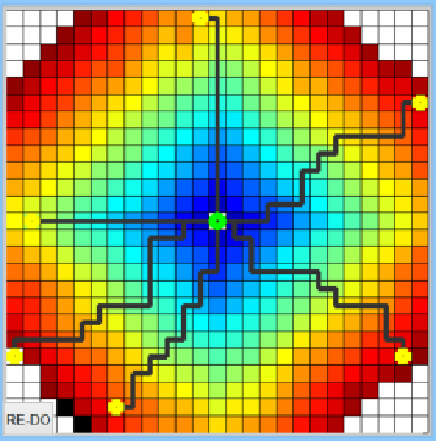
\includegraphics[width=0.7\textwidth]{img/mg-biddfs}
		\caption{více cílové BIDDFS hledající 6 cílů (Lim, 2015)}
		\label{fig:mg-biddfs}
	\end{figure}
	
	
	\newpage
	
	\section*{Porovnaní}
	
	Prezentovaný algoritmus byl otestován a porovnán s jeho vlastníma variantami a i s několika jinými pathfinding algoritmy. Algoritmy byli testování na počítači s Intel Core i7 3770K 3.9 GHz, s 16GB DDR3 RAM používající Windows 8.1 a implementované v Mathworks MATLAB 2013a 64-b (Lim, 2015). V měření byl zaznamenáván čas hledání cesty a jaké hodnoty nabývala hraniční hodnota při ukončení algoritmu, čím vyšší hraniční hodnota, tak tím více uzlů bylo prohledáno. Každý algoritmus byl spuštěn několikrát na mapách s různým procentem překážek. 
	
	V Tabluce \ref{tab:biddfs} na straně \pageref{tab:biddfs} je měřena rychlost BIDDFS na různě velikých mapách s různým procentem překážek. Je vidět že s vyšším procentem překážek výrazně klesá čas hledání cíle a hraniční hodnota.

\begin{table}[h]
	\centering
	\begin{tabular}{c|c|c|c}
		\hline
		Rozměr mapy & Procento překážek & Čas hledání, s & Hraniční hodnota \\
		\hline
		10 & 40 & 0.137 & 60 \\
		25 & 20 & 5.902 & 404 \\
		25 & 40 & 1.670 & 228 \\
		25 & 60 & 0.689 & 152 \\
		50 & 20 & 138.310 & 2044 \\
		50 & 40 & 78.249 & 1587 \\
		50 & 60 & 10.878 & 613 \\
		70 & 20 & 609.398 & 4003 \\
		70 & 40 & 362.229 & 3210 \\
		70 & 60 & 11.353 & 618 \\
		\hline
	\end{tabular}
	\caption{Výkonnostní míry BIDDFS (Lim, 2015).}
	\label{tab:biddfs}
\end{table}

Z tabulky \ref{tab:biddfsvs} na straně \pageref{tab:biddfsvs} je vidět že při zvýšení počtu překážek je BIDDFS rychlejší než informovaný algoritmus IDA* (Korf, 1988). Zrychlení přichází díky tomu že se zvýšeným počtem překážek BIDDFS nemusí každý uzel rozšiřovat do všech stran. Rozšíření jednoho uzlu bude pak v průměru rychlejší než u algoritmu IDA*.

\begin{table}[h]
	\centering
	\begin{tabular}{c|c|c|c}
		\hline
		Procento překážek & algoritmus & Čas hledání, s & Hraniční hodnota \\
		\hline
		20 & IDDFS & 7.701 & 404 \\
		20 & IDA* & 1.700 & 177 \\
		20 & Dijkstra’s & 0.814 & -- \\
		20 & BIDDFS & 5.092 & 404 \\
		\hline
		60 & IDDFS & 1.183 & 152 \\
		60 & IDA* & 0.973 & 140 \\
		60 & Dijkstra’s & 0.339 & -- \\
		60 & BIDDFS & 0.689 & 152 \\
		\hline
	\end{tabular}
	\caption{Porovnání různých algoritmů na mapě s různými procenty překážek.}
	\label{tab:biddfsvs}
\end{table}
	
	
	V tabulce \ref{tab:bd-biddfs} na straně \pageref{tab:bd-biddfs} je porovnání IDDFS, BIDDFS a obousměrného BIDDFS. Z výsledků je vidět že obousměrné prohledávání bude vždy efektivnější.
	
\begin{table}[h]
	\centering
	\begin{tabular}{c|c|c|c|c}
		\hline
		Rozměr mapy & Procento překážek & Algoritmus & Čas hledání, s & Hraniční hodnota \\
		\hline
		25 & 25 & IDDFS & 6.581 & 473\\
		25 & 25 & BIDDFS & 6.962 & 473\\
		25 & 25 & obousměrný BIDDFS & 0.905 & 166\\
		\hline
		25 & 40 & IDDFS & 5.622 & 407\\
		25 & 40 & BIDDFS & 5.366 & 407\\
		25 & 40 & obousměrný BIDDFS & 0.741 & 139\\
		\hline
		25 & 60 & IDDFS & 0.952 & 178\\
		25 & 60 & BIDDFS & 0.930 & 178\\
		25 & 60 & obousměrný BIDDFS & 0.303 & 87\\
		\hline
		70 & 25 & IDDFS & 509.844 & 3770\\
		70 & 25 & BIDDFS & 514.783 & 3770\\
		70 & 25 & obousměrný BIDDFS & 69.083 & 1415\\
		\hline
		70 & 40 & IDDFS & 322.398 & 3064\\
		70 & 40 & BIDDFS & 316.537 & 3064\\
		70 & 40 & obousměrný BIDDFS & 64.610 & 1362\\
		\hline
		70 & 60 & IDDFS & 7.252 & 489\\
		70 & 60 & BIDDFS & 7.003 & 489\\
		70 & 60 & obousměrný BIDDFS & 2.239 & 203\\
		\hline
	\end{tabular}
	\caption{Porovnání obousměrného BIDDFS s ostatními algoritmy (Lim, 2015).}
	\label{tab:bd-biddfs}
\end{table}

	V dalším testování byli měřeny obousměrné BIDDFS a paralelní obousměrné BIDDFS. Z výsledků je vidět že díky vláknu, které pouze sleduje jestli se cesty potkali, bylo ušetřeno jedno zvýšení hraniční hodnoty, ale k dramatickému ušetření času nedošlo. Při rozloze mapy 70x70 paralelní obousměrný BIDDFS ušetřil o proti jeho neparalelní verzi pouze 1s.

\begin{table}[h]
	\centering
	\begin{tabular}{c|c|c|c}
		\hline
		Rozměr mapy & Algoritmus & Čas hledání, s & Hraniční hodnota \\
		\hline
		25 & paralelní obousměrné BIDDFS & 0.959 & 168 \\
		25 & obousměrné BIDDFS & 1.098 & 169 \\
		\hline
		70 & paralelní obousměrné BIDDFS & 15.977 & 672 \\
		70 & obousměrné BIDDFS & 16.893 & 673 \\
		\hline
	\end{tabular}
	\caption{Porovnání obousměrného BIDDFS a paralelního obousměrného BIDDFS (Lim, 2015).}
	\label{tab:bbiddfsvspbbiddfs}
\end{table}

	\newpage

 	V posledním měření je porovnán klasický BIDDFS s více cílovým BIDDFS. Výsledky testování jsou v tabulce \ref{tab:mg-biddfs} na straně \pageref{fig:mg-biddfs}. Z výsledků je vidět že při hledání více cílů v jedné mapě upravený BIDDFS ušetří spoustu času o proti klasickému BIDDFS, který po nalezení každého cílu musí začít novou iteraci od počátečního uzlu, proti tomu více cílový BIDDFS mapu prochází pouze jednou dokud nenalezne všechny cíle.	
 	
 	\begin{table}[h]
 		\centering
 		\begin{tabular}{c|c|c|c|c}
 			\hline
 			Počet cílů & Algoritmus & Čas hledání, s & Hraniční hodnota & Počet opakování\\
 			\hline
 			2 & BIDDFS & 12.652 & 782 & 2\\
 			2 & více cílový BIDDFS & 10.142 & 550 & 1\\
 			\hline
 			4 & BIDDFS & 28.475 & 1725 & 4\\
 			4 & více cílový BIDDFS & 10.561 & 550 & 1\\
 			\hline
 			6 & BIDDFS & 41.477 & 2562 & 6\\
 			6 & více cílový BIDDFS & 10.774 & 550 & 1\\
 			\hline
 		\end{tabular}
 		\caption{Porovnání BIDDFS a více cílového BIDDFS (Lim, 2015).}
 		\label{tab:mg-biddfs}
 	\end{table}
	
	\section*{Závěr}
	
	V tom referátu je prezentován algoritmus BIDDFS a jeho různé varianty. Z testování lze vyvodit, že BIDDFS je v každém případě efektivnější než algoritmus IDDFS ze kterého vychází. Při vyšším procentu překážek v mapě BIDDFS dokáže překonat v rychlosti i algoritmus IDA*, ale i přes snížení redundance prohledávání, BIDDFS je stále neefektivní v mapách kde jsou žádné nebo málo překážek. Dále navrhovaný obousměrný BIDDFS byl testováním prokázán jako rychlejší verzí klasického BIDDFS a pomocí rozdělení do více vláken tento algoritmus může být ještě více optimalizován. Nakonec byl představen více cílový BIDDFS a testováním bylo prokázáno že pokud hledáme v jedné mapě více cílů, tak několikanásobně snižuje redundanci prohledávání a redukuje dobu hledání než kdybychom pro každý cíl zvlášť spouštěli klasický BIDDFS.
	
	
	\section*{Reference}
	
	Dijkstra, E. W. (1959). A note on two problems in connexion with graphs.
	Numerische Mathematik, 1(1), 269–271.
	
	Korf, R.E. (1985) ‘Depth-first iterative-deepening’, Artificial Intelligence, 27(1), pp. 97–109. doi:10.1016/0004-3702(85)90084-0.
	
	Korf, R.E. (1988) ‘Optimal path-finding algorithms’, Search in Artificial Intelligence, pp. 223–267. doi:10.1007/978-1-4613-8788-6\_7. 
	
	Lim, K.L. et al. (2015) ‘Uninformed pathfinding: A new approach’, Expert Systems with Applications, 42(5), pp. 2722–2730. doi:10.1016/j.eswa.2014.10.046.
	
	
	
\end{document}
